\section{Fluxograma do jogo}
\section{Funcionalidades}
\subsection{Menu}
\subsection{Modo Corrida}
\label{corrida}
\subsection{Modo Livre}
\label{livre}
\subsection{Controle da Bicicleta}
\subsection{Física do Jogo}
\subsection{Conta}
\subsection{Gráficos}

\subsection{Personagens}
A visão do jogador consiste na orientação da câmera que representa o \textit{Oculus}. Dentro do jogo é a visão do personagem, no qual está posicionado em cima da bicicleta, para proporcionar a sensação de imersão. É possível visualizar a movimentação do personagem como o pedalar de acordo com a velocidade, os braços acompanhando a direção do guidão, entre outras. Existem dois tipos de personagens no jogo que podem ser selecionados pelo jogador: um homem e uma mulher, demonstrados na Figura \ref{figura:mulher} e Figura HOMEM. 

\begin{center}
	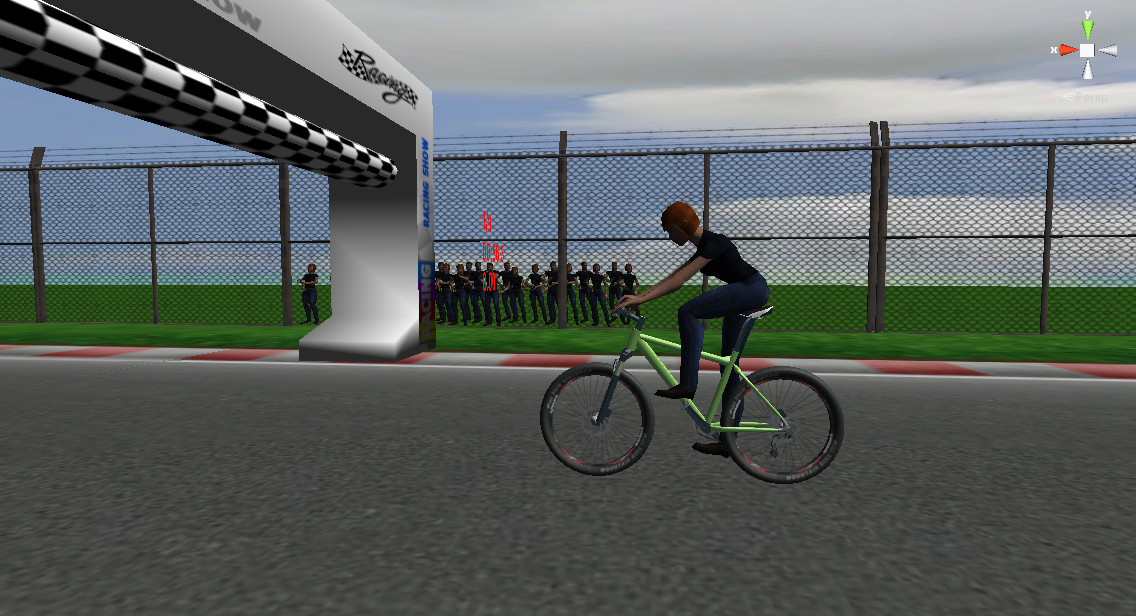
\includegraphics[scale=0.4]{figuras/mulher}
	\captionof{figure}{Personagem feminina vista de perfil.}
	\label{figura:mulher}
\end{center}

\subsection{Cenários}

O jogador poderá escolher opções do cenários para jogar como:

\begin{description}
\item[Pistas] Uma pista íngreme e uma pista regular.
\item[Modo Corrida e Modo Livre] Detalhados nas Seções \ref{corrida} e \ref{livre}.
\item[Noturno e Diurno] Cenário noturno (Figura \ref{figura:noturno}) com os postes ligados, lua e estrelas e o cenário diurno (Figura \ref{figura:diurno}) com nuvens, sol e postes desligados.
\end{description}

\begin{center}
	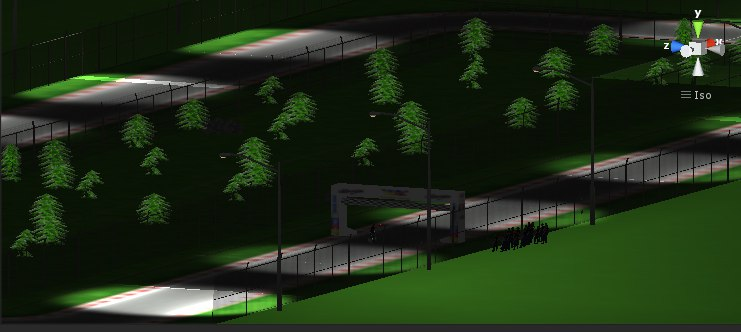
\includegraphics[scale=0.4]{figuras/noturno}
	\captionof{figure}{Cenário noturno.}
	\label{figura:noturno}
\end{center}

\begin{center}
	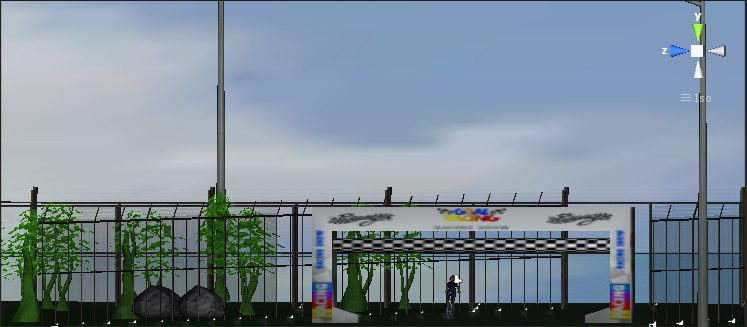
\includegraphics[scale=0.4]{figuras/diurno}
	\captionof{figure}{Cenário diurno.}
	\label{figura:diurno}
\end{center}

As imagens abaixo contém os elementos principais que compõem o cenário do jogo.

\begin{center}
	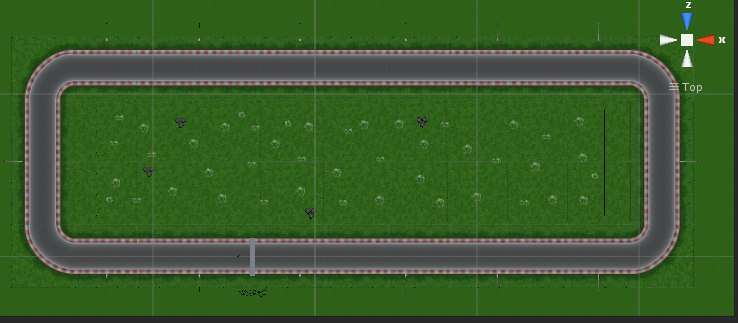
\includegraphics[scale=0.4]{figuras/pista}
	\captionof{figure}{Vista superior da pista regular.}
	\label{figura:pista}
\end{center} 

\begin{center}
	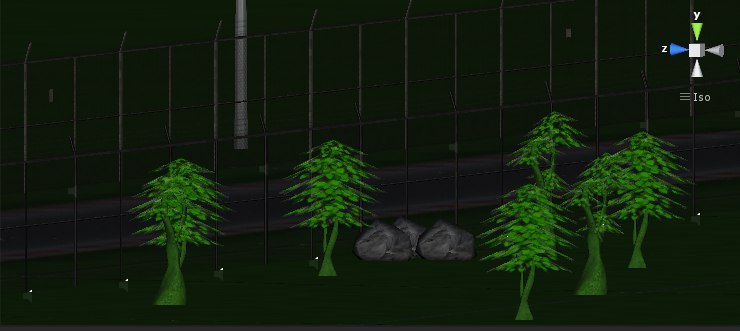
\includegraphics[scale=0.4]{figuras/jardim}
	\captionof{figure}{Jardim localizado no centro do cenário.}
	\label{figura:jardim}
\end{center}


\begin{center}
	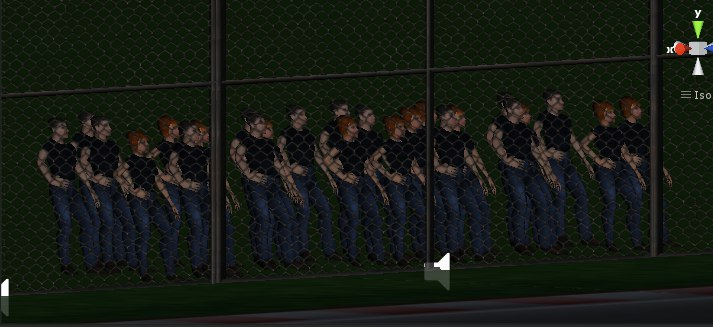
\includegraphics[scale=0.4]{figuras/torcida}
	\captionof{figure}{Torcida localizada proximo à linha de chegada.}
	\label{figura:torcida}
\end{center}

\begin{center}
	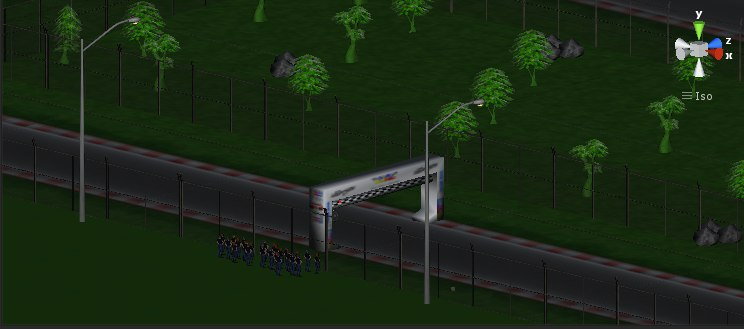
\includegraphics[scale=0.4]{figuras/visaocima}
	\captionof{figure}{Visão próxima á linha de chegada.}
	\label{figura:visaodecima}
\end{center}

\section{Arquitetura}

\subsection{Modelo de domínio}

\subsection{Arquitetura de componentes}

\subsection{Fluxo de Informa\c{c}ões}
\subsubsection{MQTT}

O MQTT é um protocolo baseado em mensagens utilizado em soluções IOT. Como ilustrada na Figura \ref{figura:mqttsoft}, o MQTT possui três papéis principais para o estabelecimento das trocas de mensagens: o \textit{Broker}, o \textit{Publisher} e o \textit{Subscriber}: O \textit{Broker} é um servidor responsável por intermediar o recebimento e envio das mensagens e é onde é implementado toda a lógica responsável pelo armazenamento de dados. O \textit{Publisher} é o dispositivo que mandará mensagens em tópicos para o Broker de modo que fique acessível para o \textit{Subscriber} ler a mensagens.

A identificação das mensagens é definida por tópicos que podem ser identificadas por palavras divididas por barras, como por exemplo: \textit{\textbf{bike/velocity}}. Para que o \textit{Publisher} publique uma mensagem, o tópico deve ser definido. E para que o \textit{Subscriber} leia a mensagem, ele se inscrever no tópico desejado. Os dados contidos nas mensagens trocadas pelo MQTT estão em \textit{bytecode}.
    
\begin{center}
	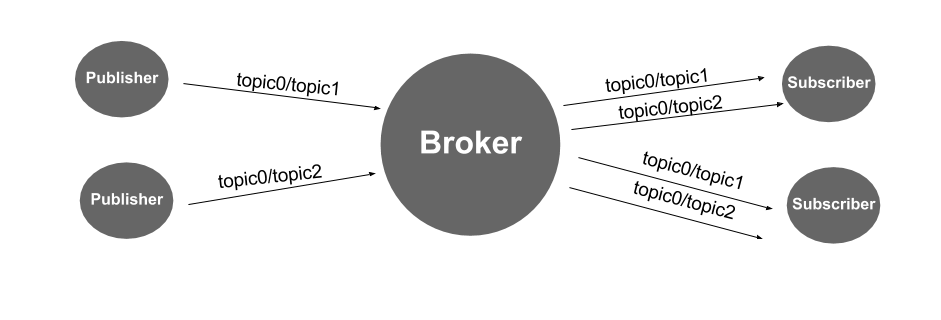
\includegraphics[scale=0.4]{figuras/MQTT}
	\captionof{figure}{Fluxo de mensagens do MQTT.}
	\label{figura:mqttsoft}
\end{center} 

    
Neste projeto, o jogo agirá como um \textit{Publisher} e como um \textit{Subscriber}. Por exemplo, para definir a velocidade da bicicleta e a angulação do guidão, agirá como um \textit{Subscriber} e para definir a angulação vertical, agirá como um \textit{Publisher}. As funções de publicação, inscrição, conexão, entre outras é importada do asset do MQTT disponível para Unity.  A classe que faz as intermediações entre os dados no jogo é a \textit{InputOutput} que será detalhada no tópico a seguir.

\subsubsection{\textit{InputOutPut} e \textit{Mock} do \textit{Input}}

Na função \textit{Start} da classe  \textit{InputOutput}, é realizada a conexão do jogo com o \textit{Broker} através do IP e porta e a inscrição de todos os tópicos que serão utilizados. Os tópicos presentes atualmente são: o \textit{bike/velocity} para a velocidade da bicicleta e o \textit{bike/angle} para a angulação do guidão. 

Como a integração com o sistema físico ainda não foi realizada, é implementado um \textit{Publisher} para enviar mensagens a partir de eventos do teclado. Portanto, para testes do subsistema isolado, o fluxo de informações é o seguinte: 

\begin{itemize}
\item Quando a seta ${\uparrow}$ é pressionada, é enviado uma mensagem através de um Publish que a tecla está sendo pressionada no tópico \textit{bike/velocity} . No \textit{script} responsável pelo controle do movimento da bicicleta, são repassadas as mensagens contidas no tópico de velocidade que aumenta gradativamente enquanto esta tecla estiver pressionada.
\item Quando as setas ${\leftarrow}$ e ${\rightarrow}$ são pressionadas, também é enviado uma mensagem através de um \textit{Publish} que a tecla está sendo pressionada no tópico \textit{bike/angle}. As mensagens contidas no tópico de angulação são repassadas para o script responsável pela movimentação e é variada então em 45$^{\circ}$  para direita ou esquerda dependendo da tecla pressionada e para 0$^{\circ}$  quando nenhuma das duas estiver pressionada.
\item Concluindo, o \textit{Publisher} que é acionado através do \textit{Input.GetKey}, uma espécie de handler de eventos do teclado,  envia dados para o \textit{Broker} que repassa para o jogo como demonstrado na Figura \ref{figura:inputoutput}.
\end{itemize}

\begin{center}
	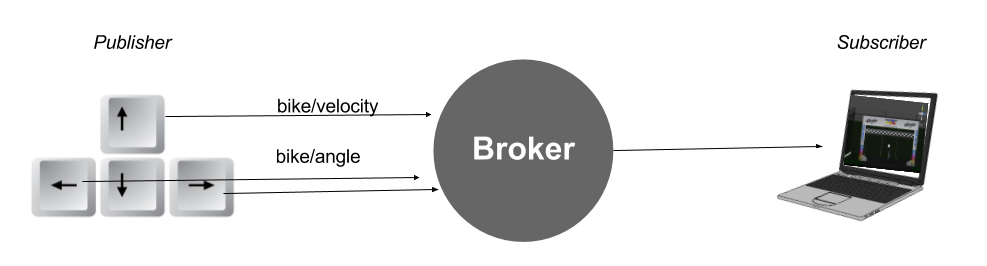
\includegraphics[scale=0.4]{figuras/inputoutp}
	\captionof{figure}{Integração através do MQTT}
	\label{figura:inputoutput}
\end{center} 

\subsection{Banco de Dados}
Para o armazenamento das informações relativas a conta de um usuário foi adotado a utilização de um banco de dados. Tais informações incluem sendo tanto os dados pessoais como, nome, altura e peso, quanto os dados relativos ao desenvolver do usuário, como o tempo das voltas, batimentos cardíacos durante a corrida, frequência respiratória e velocidade no circuito, entre outros, que poderão vir a ser adicionados para melhorar a funcionalidade de estatísticas.

O banco de dados escolhido foi o \hyperref[iBoxBD]{'http://www.iboxdb.com/''}, uma banco de bados totalmente não relacional, que é leve e usa pouca memória. Ele é executado como um servidor incorporado como banco de dados local, também suporta conexão de conexão TCP como parte do sistema distribuído. Outras vantagens são: único arquivo, ausência da necessidade de configuração e suporte ao C\#. 
	
Na implementação dele no projeto foi criado um Singleton, que instância e gerencia a “Box”, que é parte desse BD que cuida do contexto das operações e as executa. Além disso foi criada uma DAO para o Player, que separa as regras de negócio do jogo do acesso aos dados, que se dá pelo Singleton. O Player, por sua vez, possui todas as informações que se refere a ele e que vai adquirindo, já citadas anteriormente.
